
\begin{figure}
    \centering
    \begin{subfigure}{.47\textwidth}
        \centering
        %\includegraphics[width=0.9\linewidth]{lizard-2.jpg}
        %
\includegraphics[width=0.9\linewidth]{lizard-crop-birds.jpg}
        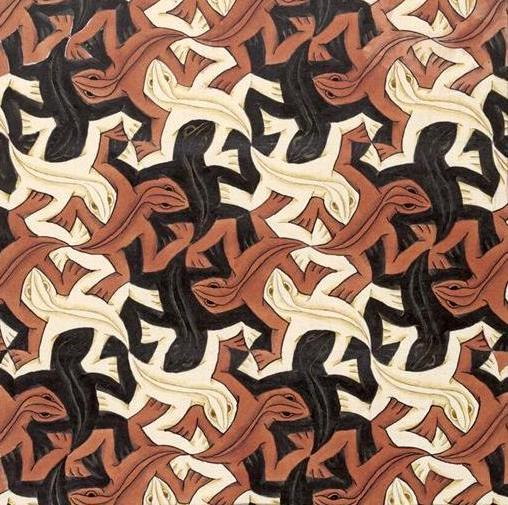
\includegraphics[width=0.9\linewidth]{lizard-crop-horseman.jpg}
        \caption{Lizard tiling \cite{m.c.escherLizard1942}}
        \label{fig:tiling_three}
    \end{subfigure}\quad
    \begin{subfigure}{.47\textwidth}
        \centering
        %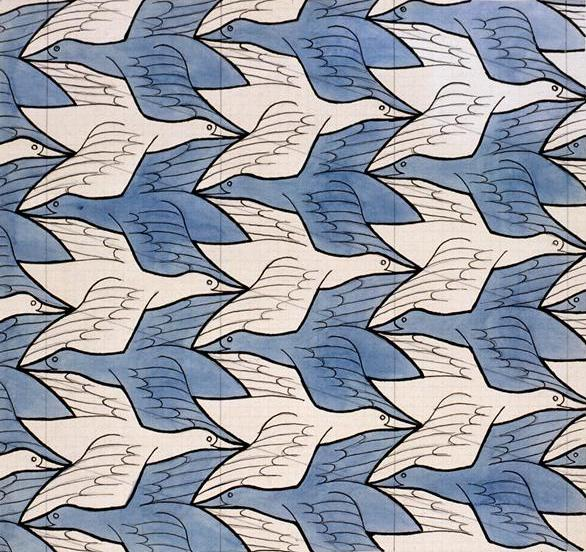
\includegraphics[width=0.9\linewidth]{two-birds-1.jpg}
        
\includegraphics[width=0.9\linewidth]{horseman-1.jpg}
        \caption{Horseman tiling \cite{m.c.escherHorseman1946}}
        %\caption{Horseman tiling}
        \label{fig:tiling_four}
    \end{subfigure}
    \caption{Two monohedral tilings of the plane using a Lizard- and a Horseman-shaped tile, respectively. Both \cref{fig:tiling_three,fig:tiling_four} are made by artist M. C. Escher. Although the coloring of both the lizards and horsemen is different, they are all the same tile. Furthermore, in addition to using translation, \cref{fig:tiling_three} tile by rotation, and \labelcref{fig:tiling_four} tile by reflection.}
    \label{fig:tilings_three_four}
\end{figure}



\mycomment{  %! Block comment
\begin{figure}[t]%h!
    \centering
    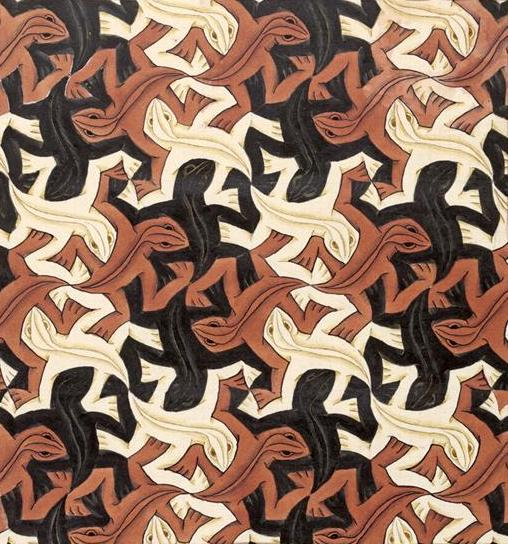
\includegraphics[width=0.4\linewidth]{lizard-1.jpg}
    \caption{A monohedral tiling of the plane using a Lizard-shaped tile by artist M.C Escher \cite{m.c.escherLizard1942}. Although the lizards are colored differently, they are, in fact, the same tile. Although the coloring of the lizards is different, they are all the same tile.}
    %\label{fig:tiling_three}
\end{figure}
}

\mycomment{  %! Block comment
\begin{figure}[t]%h!
    \centering
    \begin{subfigure}{.47\textwidth}
        \centering
        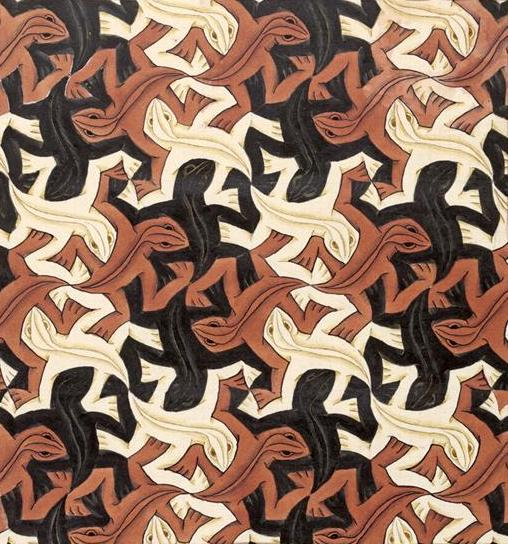
\includegraphics[width=0.9\linewidth]{lizard-1.jpg}
        \caption{Lizard}
        %\label{fig:tiling_three}
    \end{subfigure}\quad
    \begin{subfigure}{.47\textwidth}
        \centering
        
\includegraphics[width=0.9\linewidth]{flying-fish.jpg}
        \caption{Flying fish}
        %\label{fig:tiling_four}
    \end{subfigure}
    \caption{from \cite{m.c.escherLizard1942}}
    %\label{fig:tilingsss_two}
\end{figure}
}

